% ============================================================
%  Section 4 — Implémentation du pipeline
% ============================================================

\section{Implémentation du pipeline}
\label{sec:pipeline}

Chaque étape du pipeline est un module indépendant et testable, avec une interface
d'entrée/sortie explicite. Cette modularité permet de substituer une composante
sans réentraîner le reste du pipeline — condition indispensable pour les expériences
d'ablation et de comparaison d'architectures.
L'ensemble du pipeline compte 302 tests unitaires et passe le lint Ruff et mypy sans erreur.

\subsection{Étape 0 — Détection de drift (MMD-RFF)}
\label{sec:drift}

La détection de drift s'appuie sur la statistique MMD² (Maximum Mean Discrepancy)
estimée via Random Fourier Features \cite{gretton2012}, avec une complexité $O(nD)$
où $D = 256$ est le nombre de features aléatoires. Cette approximation permet
une inférence en temps réel sur des fenêtres glissantes de signaux multivariés.

Le seuil $\varepsilon_\text{drift} = 0.5226$ est calibré par critère de Youden sur les
épisodes d'entraînement contenant des drifts bénins injectés (AUC $= 0.60$ sur train).
Ce niveau d'AUC modeste reflète la difficulté intrinsèque de la détection de drift
sur des épisodes courts — le DriftDetector a davantage valeur d'indicateur complémentaire
que de détecteur primaire.

\begin{figure}[h]
\centering
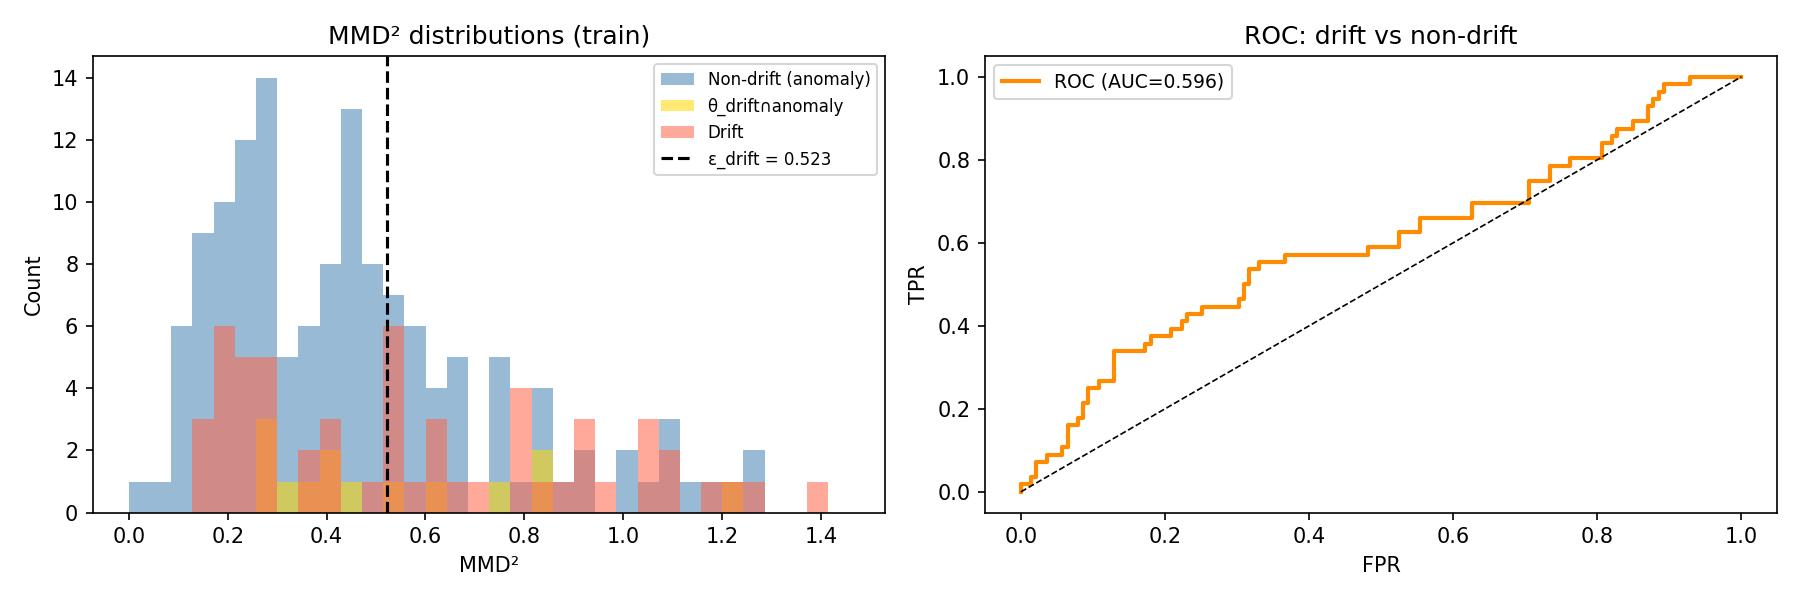
\includegraphics[width=0.80\linewidth]{figures/mmd2_distributions.png}
\caption{Distributions de $\widehat{\text{MMD}}^2$ sur le jeu d'entraînement.
  Drifts bénins (bleu) vs anomalies (orange). Le seuil $\varepsilon_\text{drift} = 0.5226$
  est calibré par critère de Youden (AUC\,=\,0.60).}
\label{fig:mmd2}
\end{figure}

Le mécanisme \emph{look-through} \cite{hinder2024} transmet le signal même lorsqu'un drift
est détecté, en lui attachant un flag \texttt{DRIFT}. Ce comportement est essentiel pour le
régime $\theta_{\text{drift} \cap \text{anomaly}}$ : sans look-through, le signal d'anomalie
serait supprimé pendant la phase de drift du déploiement défectueux.
Trois cas sont distingués :
\begin{itemize}
  \item $\widehat{\text{MMD}}^2 < \varepsilon_\text{drift}$ : signal transmis sans flag.
  \item $\widehat{\text{MMD}}^2 \geq \varepsilon_\text{drift}$,
    confirmation positive (post-drift $\geq 3$ steps) : signal transmis avec flag \texttt{DRIFT}.
  \item $\widehat{\text{MMD}}^2 \geq \varepsilon_\text{drift}$,
    confirmation négative : recalibration ($W_\text{ref} \leftarrow W_\text{cur}$).
\end{itemize}

\subsection{Étape 1 — Encodeur STGCN}
\label{sec:encoder}

L'encodeur est un Spatio-Temporal Graph Convolutional Network \cite{yu2018} qui joint
la structure spatiale du graphe de services $G(t)$ et la dynamique temporelle
du signal $S(t)$. L'architecture combine une convolution graphique GCN sur la matrice
d'adjacence pondérée $w_E(t)$ et un réseau TCN (Temporal Convolutional Network)
sur la dimension temporelle, produisant un embedding $z_e \in \mathbb{R}^{64}$.

Les paramètres principaux sont : $d_\text{feat} = 17$, $N = 6$ nœuds,
$d_\text{hidden} = 64$, $d_\text{embed} = 64$. L'entraînement est auto-supervisé sur
100 époques, avec reconstruction du signal futur comme tâche de préentraînement.
Ce préentraînement auto-supervisé permet d'exploiter les épisodes normaux
(sans injection) pour structurer l'espace latent avant le typage contrastif.

\subsection{Étape 2 — Typage siamois}
\label{sec:typing}

Le réseau siamois apprend une distance métrique $d_\varphi$ dans l'espace des embeddings
STGCN, en utilisant les labels de scénarios Chaos Mesh comme supervision faible :
des paires d'épisodes du même scénario sont rapprochées, des paires de scénarios différents
sont éloignées. La loss contrastive minimise $d_\varphi$ pour les paires positives
et la maximise (jusqu'à une marge) pour les paires négatives.

Les embeddings projetés $\{\varphi(z_e^{(i)})\}$ sont ensuite regroupés par clustering
hiérarchique agglomératif avec linkage de Ward, $K$ étant sélectionné par maximum du
score de silhouette sur le jeu d'entraînement ($K = 10$ sur ewat\_v3).
Les labels de validation et de test sont assignés par plus proche centroïde depuis les
centroides calculés sur train — correction méthodologique essentielle pour éviter la
fuite d'information inter-splits qui existait dans une version antérieure du code.

\subsection{Étape 2b — Ontologie}
\label{sec:ontology}

L'ontologie $\mathcal{O} = (\mathcal{C}, \mathcal{R})$ encode trois types de relations
entre clusters :

\textbf{Relations temporelles.}
Une transition $C_i \to C_j$ est ajoutée si le support (nombre d'épisodes présentant
cette transition) est $\geq 3$. Cela produit 22 relations sur ewat\_v3, dont
10 auto-transitions $C_i \to C_i$ (épisodes à cluster unique) et 12 transitions inter-clusters.

\textbf{Relations causales.}
La Transfer Entropy est estimée par l'estimateur KSG (Kraskov-Stögbauer-Grassberger)
\cite{kraskov2004}, avec 100 permutations de bootstrap pour le test de significativité
et correction BH-FDR \cite{benjamini1995} pour les tests multiples.
Une distinction critique sépare l'estimateur cluster-level (qui agrège toutes les séries
temporelles d'un cluster avant d'estimer la TE — biais écologique documenté) de
l'estimateur service-level (intra-épisode, sans biais). Les résultats rapportés en
Section~\ref{sec:ontology_results} utilisent l'estimateur service-level.

\textbf{Relations de co-occurrence.}
Test $\chi^2$ Yates 2$\times$2 avec fallback Fisher exact si le nombre attendu est $< 5$,
correction Holm--Bonferroni pour les tests multiples.

\subsection{Étape 3 — Précurseurs typés}
\label{sec:precursor}

Pour chaque type $C_i$, un classifieur logistique one-vs-rest $f_i$ est entraîné
sur les embeddings de la fenêtre pré-injection $[t-k, t]$ :
\[
  \hat{p}_i(t) = f_i\!\bigl(\varphi(z_e(S_{[t-k,t]})),\, G(t)\bigr) \in [0,1]
\]

L'horizon optimal est sélectionné sur le jeu de validation :
$k^*_i = \arg\max_{k \in \{2,4,6,8,10,12\}} \text{AUROC}(f_i, k, \text{val})$,
et l'AUROC est rapporté exclusivement sur test.
Cette séparation stricte val/test évite le surapprentissage du choix d'horizon.

Lorsque $\hat{p}_i(t) >$ seuil, une alerte est émise :
$\text{Alert}(t) = (C_i,\, \hat{p}_i(t),\, k^*_i,\, \text{fiche}_{C_i})$.
La fiche $\text{fiche}_{C_i}$ contient les features les plus importantes pour ce cluster,
calculées par permutation importance et validées par KernelSHAP.

\subsection{Alertes — AlertAssembler}
\label{sec:alerts_impl}

L'AlertAssembler intègre les sorties des étapes 0, 2 et 3 en mode streaming step-by-step.
À chaque pas de temps $t$, il reçoit le signal $S(t)$, interroge le DriftDetector,
le SiameseTyper et les PrecursorClassifiers, et produit une alerte si le seuil est atteint.

Le lead time est calculé comme $\Delta t = t_\text{injection} - t_\text{première alerte}$ :
une valeur positive indique une alerte précoce. Le point opérationnel recommandé est
le seuil $0.7$, qui réduit le taux de fausses alarmes sur drifts à $8.3$\,\%
tout en maintenant un lead time moyen de $3.0$\,min (Section~\ref{sec:alerts_results}).
